\documentclass{beamer}

\usepackage{booktabs}
\usepackage{graphicx}
\usepackage{minted}
\usemintedstyle[python]{solarizedlight}
\usepackage{tikz}
\usetikzlibrary{shapes, arrows}
\usetheme{metropolis}

\usepackage[backend=biber]{biblatex}
\bibliography{PyCon}


\title{from \_\_future\_\_ import profit}
\author{James Campbell}
\institute[Cardiff University]
  {
  Department of Mathematics\\
  Cardiff University
  }
\date{PyCon UK, 2017}

\begin{document}

\begin{frame}
  \titlepage
\end{frame}



\section{What will you learn from this talk?}

\begin{frame}{What will you learn from this talk?}
  \begin{itemize}
    \item My Background
    \item CryptoCurrency Markets
    \item Why you should start trading in Python
    \item My experiences so far
  \end{itemize}
\end{frame}



\section{What will you NOT learn from this talk?}

\begin{frame}{What will you NOT learn from this talk?}
  \begin{itemize}
    \item A deep explanation of blockchain technologies
    \item Different Trading strategies
  \end{itemize}
\end{frame}



\section{Who Am I?}

\begin{frame}{Who Am I?}
  \begin{itemize}
    \item GitHub: \href{https://github.com/theref}{www.github.com/theref}
    \item Website: www.jamescampbell.org.uk
    \item Email: \href{mailto:campbellj11@cardiff.ac.uk}{campbellj11@cardiff.ac.uk}
  \end{itemize}
\end{frame}



\section{Why Bitcoin?}

\begin{frame}{Exchanges have \alert{low fees}}
  \begin{tabular}{c c c}
        
\includegraphics[width=0.3\linewidth]{images/bitfinex} & 
\includegraphics[width=0.3\linewidth]{images/coinfloor} & 
\includegraphics[width=0.3\linewidth]{images/gdax}\\
        
\includegraphics[width=0.3\linewidth]{images/poloniex} & 
\includegraphics[width=0.3\linewidth]{images/bitstamp} & 
\includegraphics[width=0.3\linewidth]{images/bitmex}
      \end{tabular}
\end{frame}


\begin{frame}{Very Young Market}
  \begin{center}
    
\includegraphics[width=0.8\linewidth]{images/pizza_tweet}\\
    Original Bitcoin Pizza Day was 22nd May, 2010 \cite{BitPizza}
  \end{center}
\end{frame}

\begin{frame}{Exchanges are \alert{always} open}
  \begin{center}
    Over 5 times longer than convential exchanges \cite{ExchOpen}
  \end{center}
\end{frame}



\section{Why Now?}

\begin{frame}{You're still a \alert{very} early backer}
\pause
  \begin{figure}
    \begin{center}
      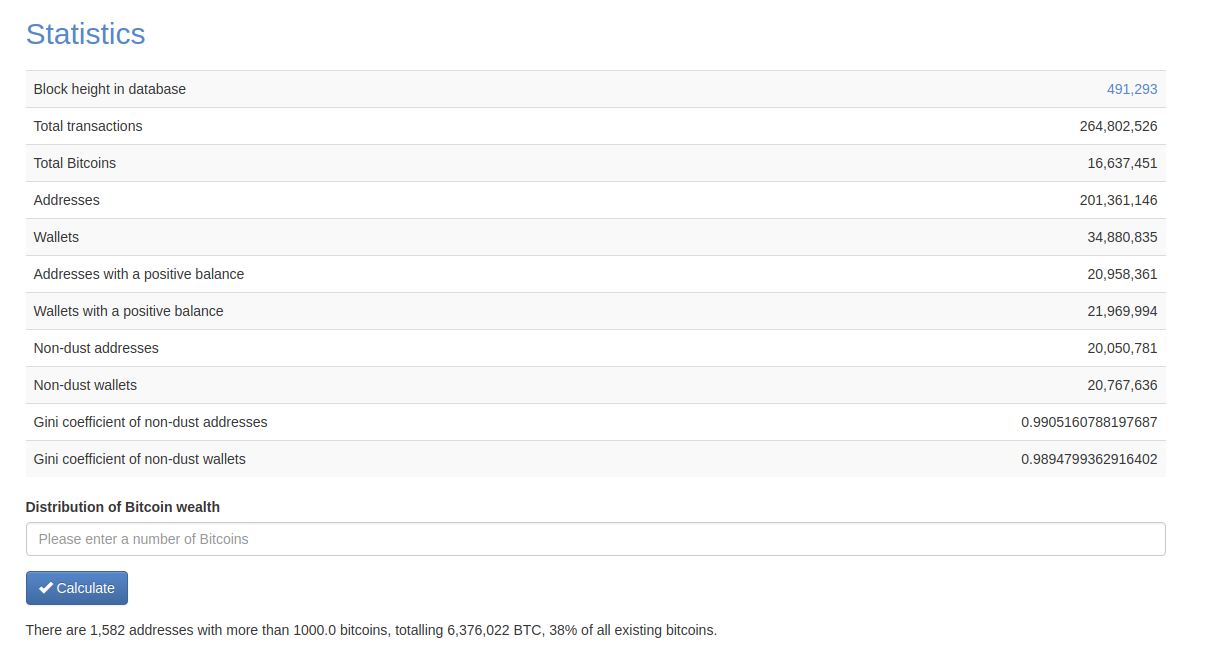
\includegraphics[scale=0.21]{images/statistics}
      \caption{Source: bitcoinprivacy.net \cite{NumAdd}}
    \end{center}
  \end{figure}
\end{frame}



\section{What Tools?}

\begin{frame}{ccxt}
  \begin{center}
    \emph{"A [Python] library for cryptocurrency trading and e-commerce with support for many bitcoin/ether/altcoin exchange markets and merchant APIs."}

    The ccxt library currently supports 91 cryptocurrency exchanges. \cite{ccxt}
  \end{center}
\end{frame}

\begin{frame}{backtrader}
  \begin{center}
    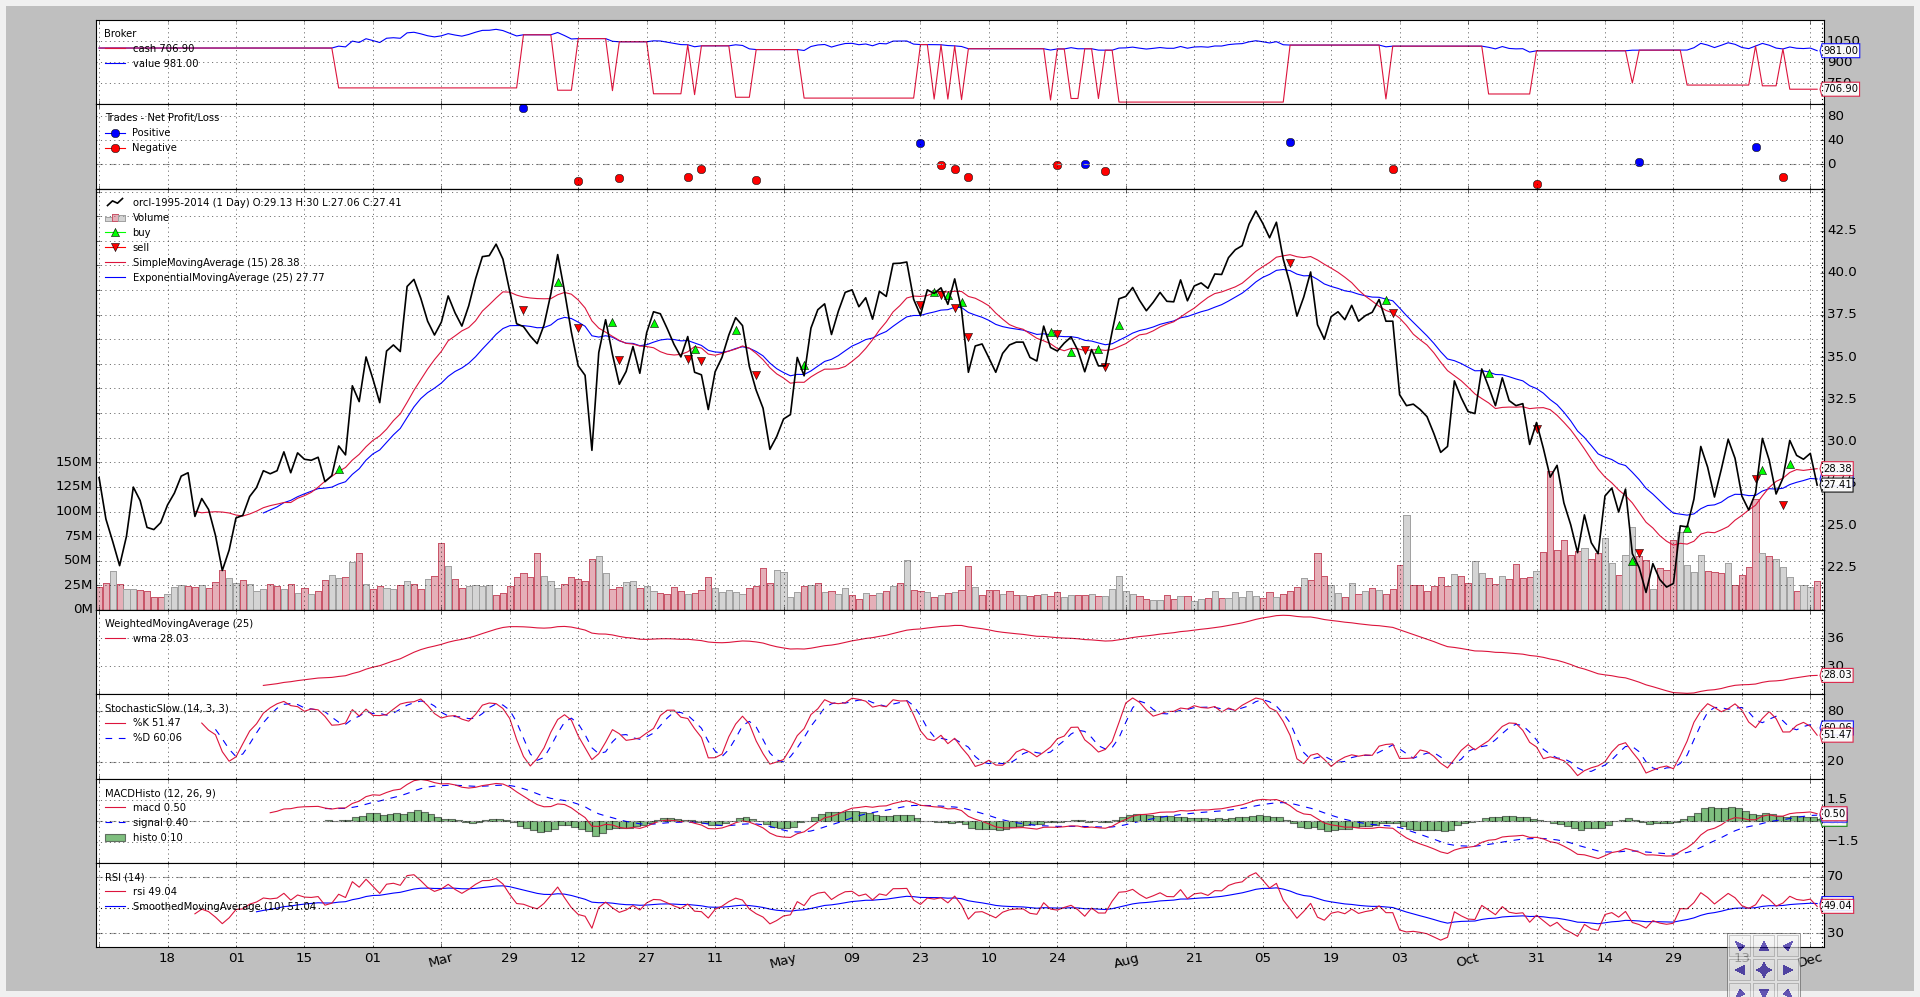
\includegraphics[scale=0.21]{images/quickstart}
  \end{center}
\end{frame}

\section{How much have I made so far?!!}

\begin{frame}{}
  \begin{center}
    {\fontsize{5cm}{5.5cm} \selectfont £0}
  \end{center}
\end{frame}

\begin{frame}[standout]
  \begin{itemize}
    \itemsep2em
    \item Email: \href{mailto:campbellj11@cardiff.ac.uk}{campbellj11@cardiff.ac.uk}

    \item GitHub: \href{https://github.com/theref}{www.github.com/theref}

    \item Twitter: \href{https://twitter.com/JamesCampbell95}{@JamesCampbell95}

    \item Website: www.jamescampbell.org.uk
  \end{itemize}
\end{frame}

\begin{frame}[allowframebreaks]
  \printbibliography
\end{frame}


\end{document}